%##########################################################################
%##########################  CHAPER 6: APPLICATION  #######################
%##########################################################################

\chapter{Entwicklung der Anwendung}\label{kap:application}

In diesem Kapitel wird die Entwicklung der Anwendung als Autonomes 
Edge System auf dem Respberry Pi zusammen mit dem Neural Compute 
Stick 2 und einer geeigneten Kamera beschrieben.
Ebenso wird die Integration des trainierten Tensorflow Models in die  
Applikation sowie die Implementierung der Neztwerk Verbindung zu dem 
System beschriebn.

%----------------------------------------------------------------------



%##########################  SECTION 1: AUFBAU  ###########################
\section{Aufbau}\label{sec:aufbau}


Die Anwendung soll auf dem ein Platinen Computer Raspberry 
Pi 4 Abbildung \ref{subfig:raspy} 
laufen, an den die nötigen Komponenten angeschlossen werden. Dazu 
ghören der Neural Compute Stick 2, zur Ausführung der Inferenz, ein 
Kamera Modul, mit welchem die Bilder aufgenommen werden, sowie ein 
WiFi Stick und Powrebank.
\\
Der Neural Compute Stick wird über USB angeschlossen und kann 
nach installation des OpenVino Toolkits \ref{sec:openvino}
 verwendet werden.
\\
Bei der Kamere handelt es sich um ein Infrarot Fähiges \textit{RaspberryPi 
Camera Module} welches zusammen mit zwei Infrarot 
LEDs montiert wird. \ref{sec:raspicam}


\begin{figure}[htb]
    \centering
    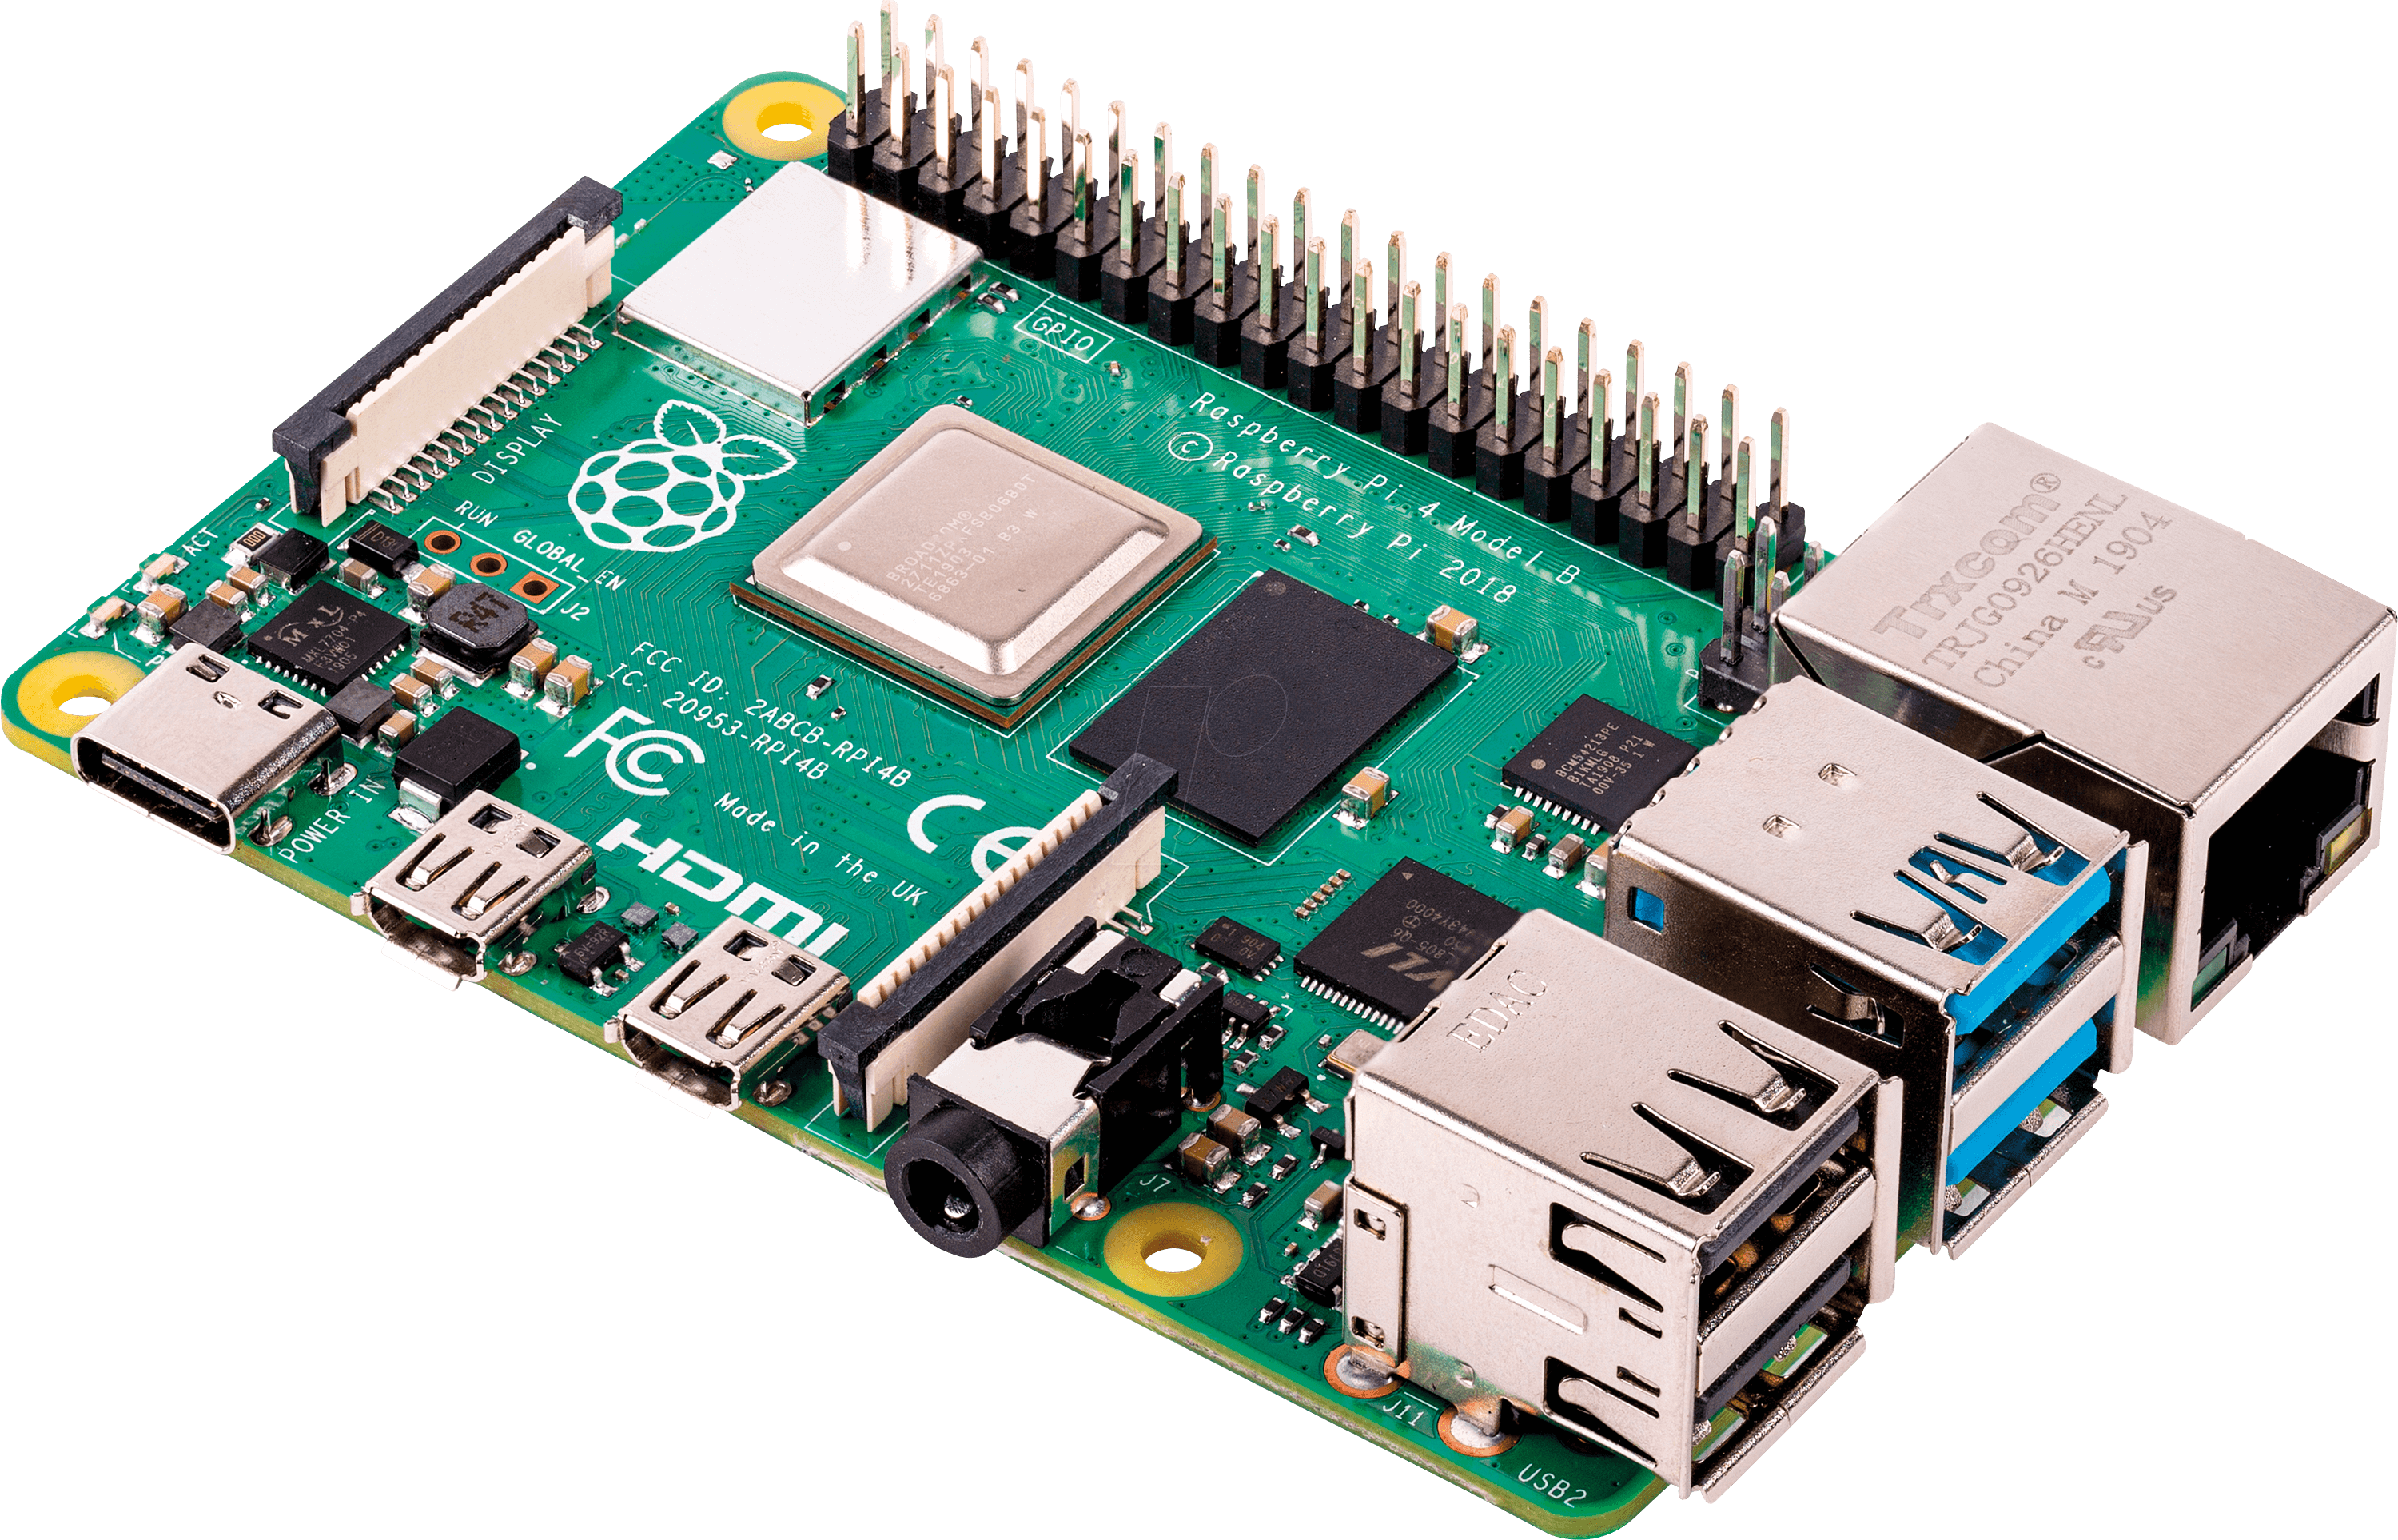
\includegraphics[width=6cm]{./Bilder/raspberrypi_4.png}
    \caption{Raspberry Pi 4}
    \label{img:raspberrypi}
\end{figure}

% \begin{figure}[htb]
%     \centering
%     \begin{subfigure}{6cm}
%         \centering
%         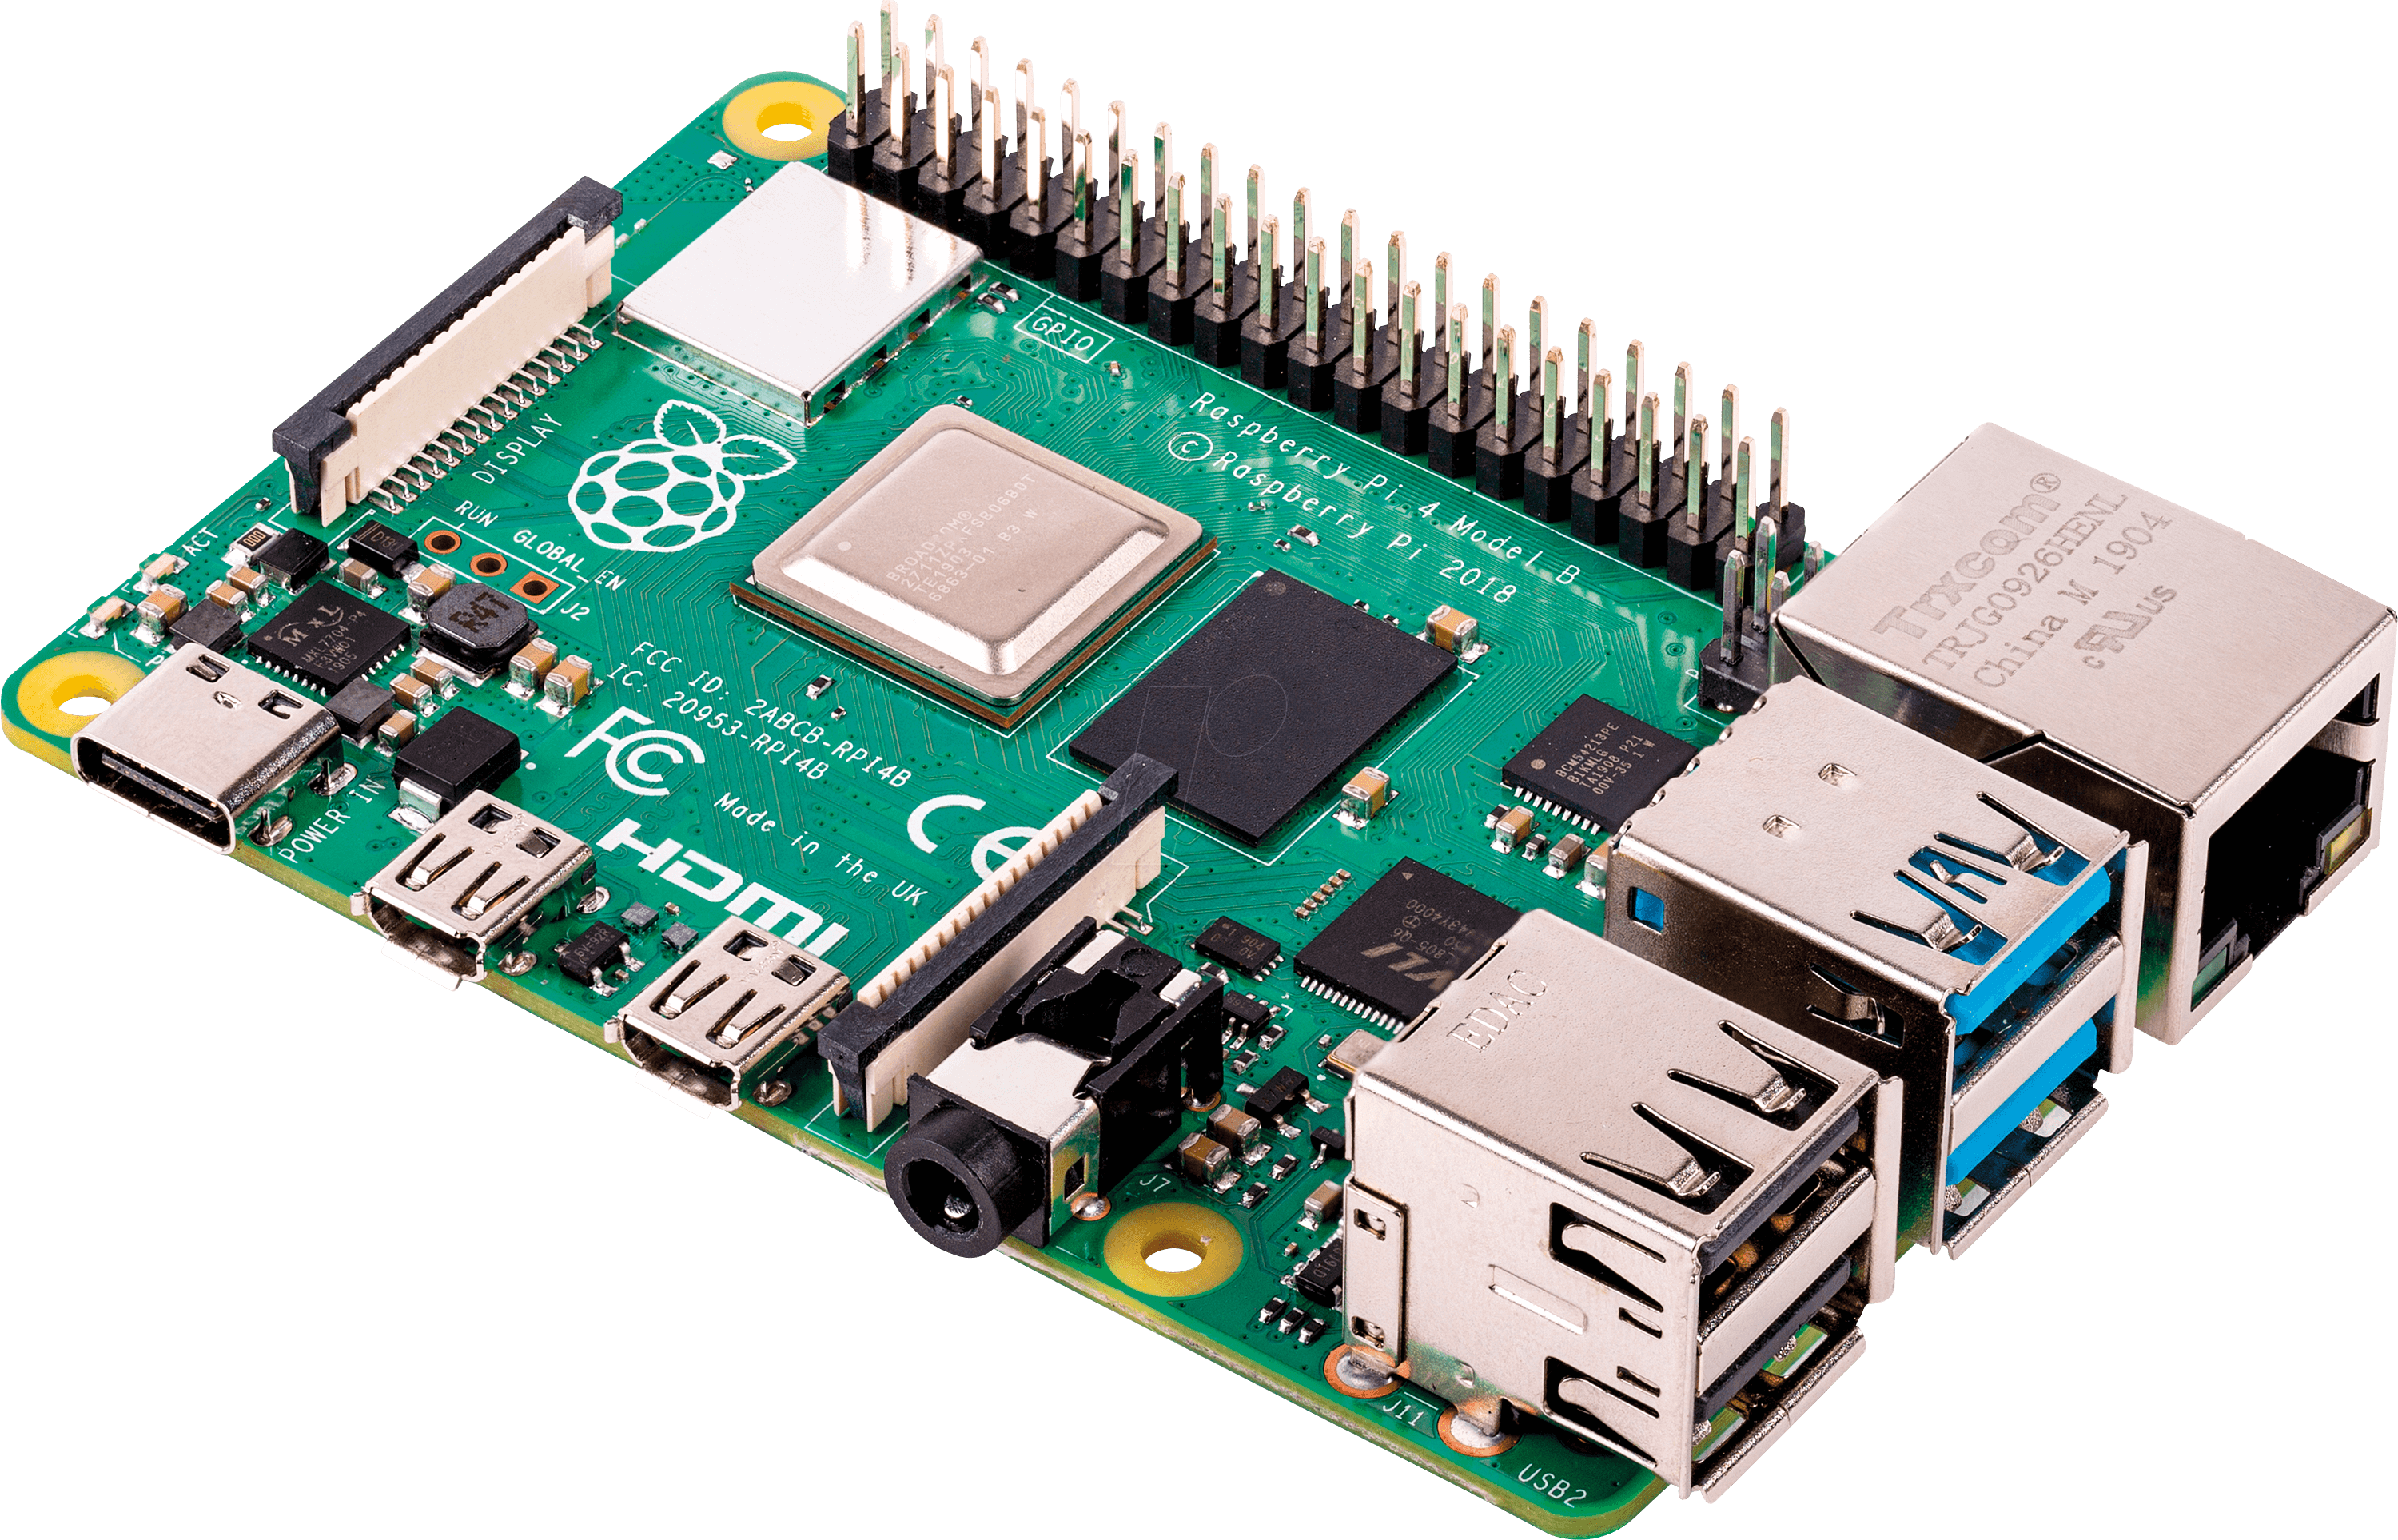
\includegraphics[width=5cm]{./Bilder/raspberrypi_4.png}
%         \subcaption{RaspberryPi 4}
%         \label{subfig:raspy}
%     \end{subfigure}
%     \begin{subfigure}{6cm}
%         \centering
%         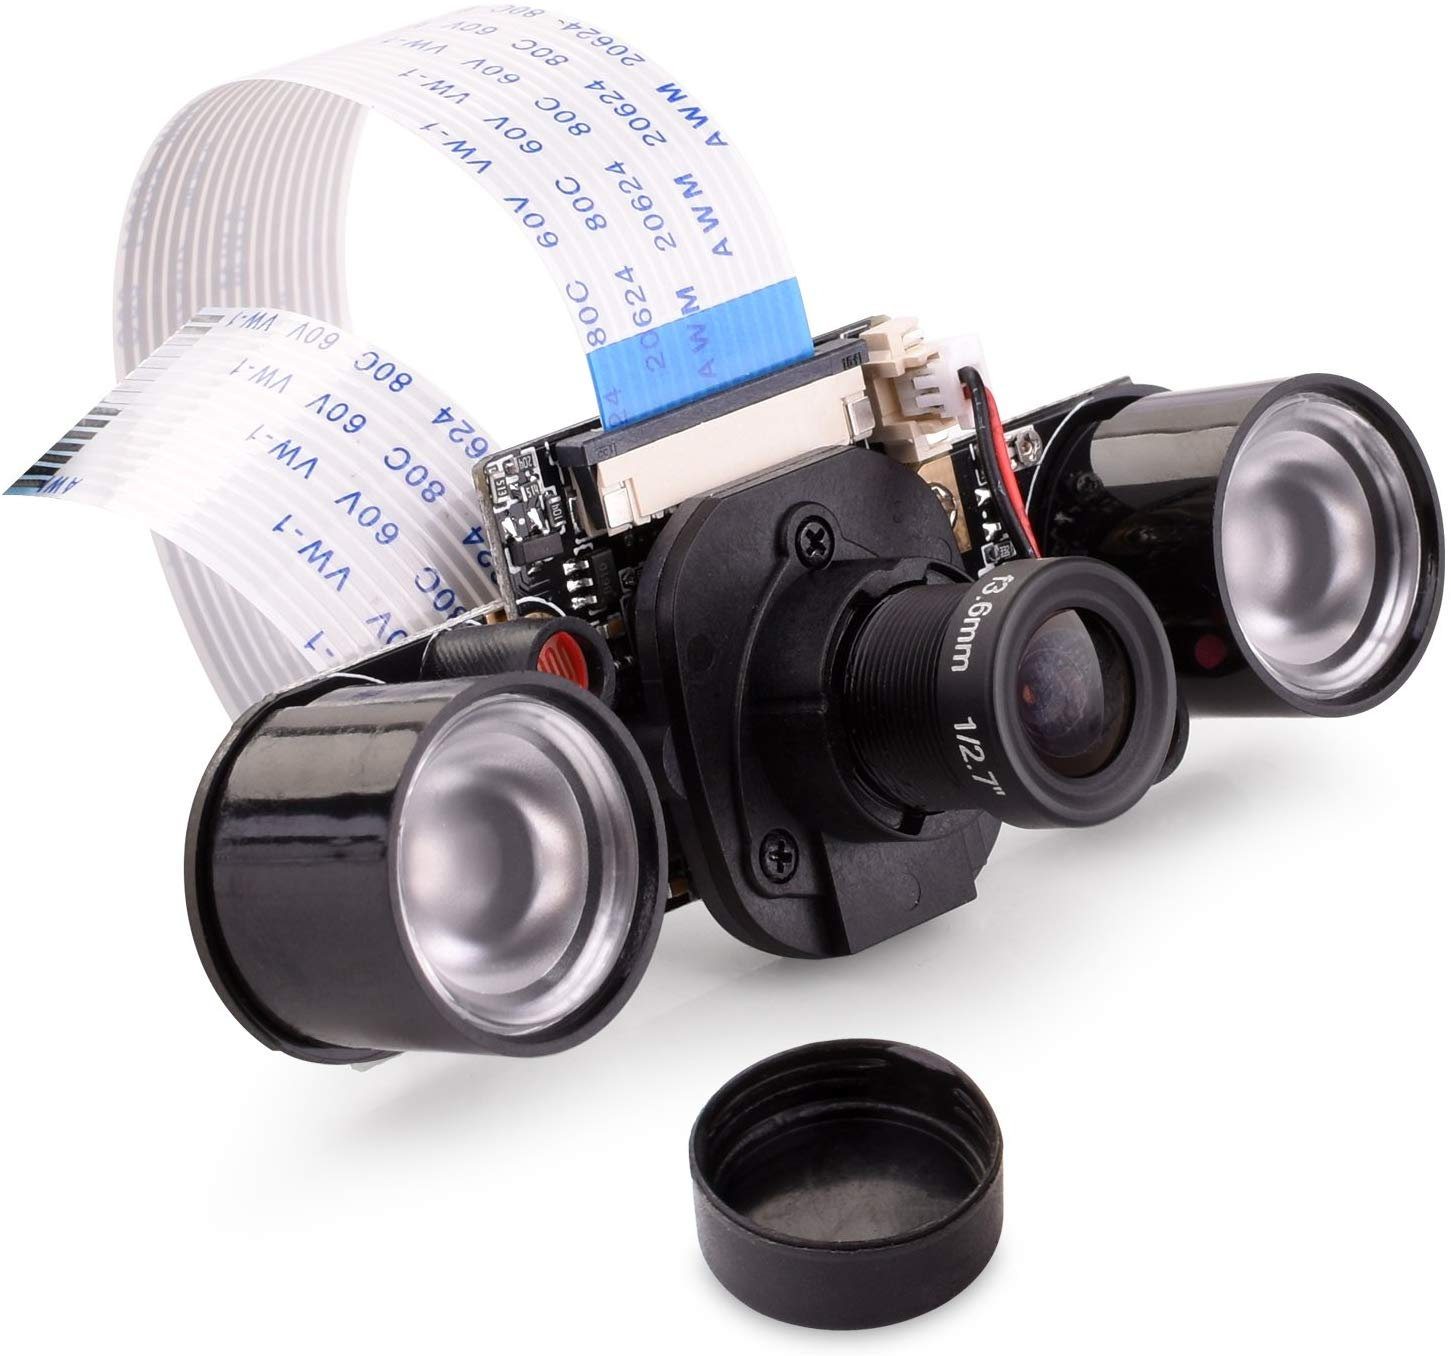
\includegraphics[width=4cm]{./Bilder/RPiCam.jpg}
%         \subcaption{Quimat Raspberry Pi Kamera}
%         \label{subfig:rpicam}
%     \end{subfigure}
%     \label{img:raspy_cam}
% \end{figure}


\begin{itemize}
    \item Netzwerkverbindzuung:
    \begin{itemize}
        \item GSM Module
        \item WiFi-Stick
    \end{itemize}
    \item Powrebank/Akku aus Sp. Verbrauch von:
    \begin{itemize}
        \item NCS2
        \item Kamera
        \item LEDs
        \item WiFi Stick
    \end{itemize}
\end{itemize}


%----------------------------------------------------------------------




%##########################  SECTION 2: OPENVINO  #######################
\section{OpenVino Toolkit}\label{sec:openvino}

% doku:
% https://docs.openvinotoolkit.org/latest/_docs_IE_DG_Introduction.html
% tutorial (mit guten diagrammen)
% Car
% https://github.com/intel-iot-devkit/inference-tutorials-generic/tree/openvino_toolkit_2019_r1_0/car_detection_tutorial#tutorial-step-3-add-the-second-model-vehicle-attributes-detection
% Face
% https://github.com/intel-iot-devkit/inference-tutorials-generic/blob/openvino_toolkit_2019_r1_0/face_detection_tutorial/Readme.md

Die Implementierung der Inferenz des trainierten Models wurde 
mithilfe des OpenVino Toolkits vorgenommen, eine Anwendung 
zur Optimierung und Ausführung von CNNs auf Intel Hardware.

Es vereinfacht und Optimiert damit die Verbindung zwischen 
Training des Models und bereitstellen in einer Anwender 
Applikation, wie in Abbildung \ref{img:openvinoworkflow} 
schematisch dargestellt.

\begin{figure}[htb]
    \centering
    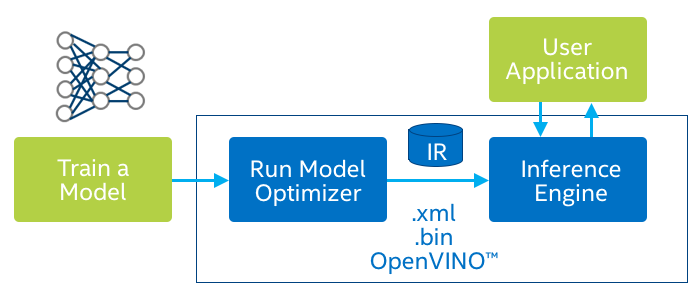
\includegraphics[width=10cm]{./Bilder/open_vino_workflow_steps.png}
    \caption{Workflow: OpenVino Toolkit}
    \label{img:openvinoworkflow}
\end{figure}

Das Toolkit besteht im Wesentlichen aus den zwei Komponenten 
\textit{Model Optimizer} und \textit{Inference Engine}

Mit dem Model Optimizer können Netze die in den Frameworks 
TensorFlow, Caffe, MXNet, Kaldi oder ONNX trainiert wurden 
in die von OpenVino verwendete Intermediate Representation 
des Modells gebracht werden.

Diese ist ein Framework unspezifisch Dateiformat, welches aus 
einer .xml Datei für die Struktur/Architektur des Modells
und einer .bin Datei fpr die trainierten gewichten besteht.


Die InferenceEngine ist eine Runtime welche eine API für die 
Sprachen C++ und Python zur Integration und Nutzung der Inferenz 
in der Anwendung bereitstellt.

Dafür werden die IR Dateien des Models in ein Hardware spezifisches 
Plugin geladen. Dieses kann die User Applikatin für die Inferenz 
von Image Classification, ObjectDetection sowie Instance Segmentation
Modellen nutzen.



%------------------------- Inference Engine ---------------------------
\subsection*{Implementierung}

Die Implementierung der Inferenz wurde in Python vorgenommen. 

Dafür waren folgende Schritte nötig:

% Als Diagramm
 
\begin{enumerate}
    \item HW Plugin laden
    \item Model IR einlesen
    \item In-Output Blobs allokieren 
    \item ausführbares Model laden
    \item inferenz request abgeben
    \item Bild als Array in Input Blob laden
    \item Inferenz
    \item Output verarbeiten, wieder zu Schritt 6
\end{enumerate}


\begin{figure}[htb]
    \centering
    
\tikzstyle{process} = [rectangle, minimum width=3cm, minimum height=1cm, text centered, draw=black]
\tikzstyle{arrow} = [thick,->,>=stealth]

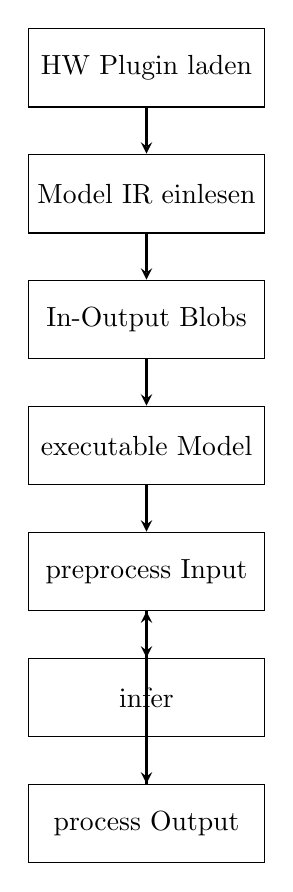
\begin{tikzpicture}[node distance=1.6cm]
    \node (hw)      [process]                   {HW Plugin laden};
    \node (ir)      [process, below of=hw]      {Model IR einlesen};
    \node (io)      [process, below of=ir]      {In-Output Blobs};
    \node (execNet) [process, below of=io]      {executable Model};
    \node (prepIn)  [process, below of=execNet] {preprocess Input};
    \node (infer)   [process, below of=prepIn]  {infer};
    \node (procOut) [process, below of=infer]   {process Output};

    \draw [arrow] (hw) -- (ir);
    \draw [arrow] (ir) -- (io);
    \draw [arrow] (io) -- (execNet);
    \draw [arrow] (execNet) -- (prepIn);
    \draw [arrow] (prepIn) -- (infer);
    \draw [arrow] (infer) -- (procOut);
    \draw [arrow] (procOut) -- (prepIn);
    
\end{tikzpicture}
    
    \label{fig:diagramm}
\end{figure}


Blobs sind In-Output Tensoren


\begin{lstlisting}[language=Python]
    plugin = IEPlugin(device='MYRIAD')
    net = IENetwork(model=model_xml, weights=model_bin)
    input_blob = next(iter(net.inputs))
    exec_net = plugin.load_network(network=net)
    infer_request = exec_net.requests[request_id]
    # bild mit opencv als numpy arra laden und von hwc nach nchw umstellen
    res = exec_net.infer(inputs={input_blop: image})
    # res enthaellt liste mit allen erkannten klassen auf dem Bild
    # fuer Objekt Detection zusaetzlich noch Bounding Box koordinaten
\end{lstlisting}


Die Inferenz kann entweder Synchron oder Asynchron ausgeführt 
werden. Der programmatische Ablauf der hier verwendeten 
asynchronen Inferenz ist im Folgenden als Pseudocode dargestellt.

% \begin{algorithm}[H]
%     \SetKwData{Current}{Current}\SetKwData{Next}{Next}
%     \While{true}{
%      capture frame\;
%      populate \Current InferRequest\;
%      \textbf{start}  \Current InferRequest\; 
%      \textbf{wait} for the \Current InferRequest\ 
%      display \Current result;
%     }
%     \caption{Synchrone Inference}
% \end{algorithm}


% von hier https://docs.openvinotoolkit.org/latest/_demos_python_demos_object_detection_demo_ssd_async_README.html
\begin{algorithm}[H]
    \SetKwData{Current}{Current}\SetKwData{Next}{Next}
    \While{true}{
     capture frame\;
     populate \Next InferRequest\;
     \textbf{start} \Next InferRequest; \tcp{asynchroner aufruf}\
     \If{\textbf{wait} for \Current done}{ \tcp{wird in eigenem  verarbeitet} \
         display \Current;
      }
      \textbf{swap} \Current and \Next InferRequests;
    }
    \caption{Asynchrone Inferenz}
\end{algorithm}


Das Ergebnis eines InferRequest für Object Detection Modelle 
enthällt eine Liste mit allen möglichen erkannten Objekten, jedes 
davon bestehend aus einem Array mit den Indices:

\begin{enumerate}
    \setcounter{enumi}{-1}
    \item batch index
    \item class label
    \item Wahrscheinlichkeit
    \item $x_{min}$ Box Koordinate
    \item $y_{min}$ Box Koordinate
    \item $x_{max}$ Box Koordinate
    \item $y_{max}$ Box Koordinate
\end{enumerate}

Mit über die Wahrscheinlichkeit ließen sich die Ergebnisse 
nach einem bestimmte Threshhold ausfiltern.\\
Die Box Koordinaten wurden in Prozent der Bild- Breit/Höhe 
angegeben wodurch sie wieder in die Original bild größe 
für die Bounding Boxes übertragen werden konnent.


%----------------------------------------------------------------------


%##########################  SECTION 3: KAMERA  ########################
\section{Raspberry Pi Kamera}\label{sec:raspicam}


Bei der Kamera handelt es sich um das OV5647 5MP Modul mit regelbarem 
Infrarotfilter. Zusammen mit zwei Infrarot LEDs von der Firma Quimat 
Abbildung \ref{subfig:rpicam}
\\
Wird der Infrarotfilter ausgeschaltet ist es durch die Infrarot LEDs mit 
850nm welligen Licht möglich auch bei dunkelheit aufnahmen zu machen, 
die in Graustufen Werten dargestellt werden.

%------------------------------------------------------------------------


%##########################  SECTION 4: CONNECTION  #####################
\section{Server-Client-Connection}\label{sec:serverclient}



%------------------------------------------------------------------------


%##########################  SECTION 1: REST  ###########################
\section{put it all together}\label{sec:ka}



%-------------------------------------------------------------------------




